\documentclass[a4paper]{report}
\usepackage[french]{babel}
\usepackage[utf8]{inputenc}
\usepackage{graphicx} %'affichage des images
\usepackage[backend=bibtex]{biblatex}
\usepackage[T1]{fontenc}
\usepackage{listings}
\usepackage{xcolor}
\usepackage{wrapfig}

\definecolor{blue}{RGB}{38, 115, 255}
\definecolor{yellow}{RGB}{166, 122, 0}
\definecolor{red}{RGB}{166, 0, 0}

\lstdefinestyle{style1}{ 
    commentstyle=\color{yellow},
    keywordstyle=\color{blue},
    stringstyle=\color{red},
    basicstyle=\ttfamily\footnotesize,
    breakatwhitespace=false,
    breaklines=true,
    keepspaces=true,
    frame=L,
    language=python,
    keepspaces=true,
    showtabs=false,
}

\lstset{escapechar=@,style=style1}

\title{Rapport projet conception logicielle}
\author{Romuald GAFFE\and Yanis COSNEFROY\and Nguyen Phuong Vy VU\and Alexandre BOURGOIN}

\date{\today}

\begin{document}

\begin{titlepage}
    \centering
    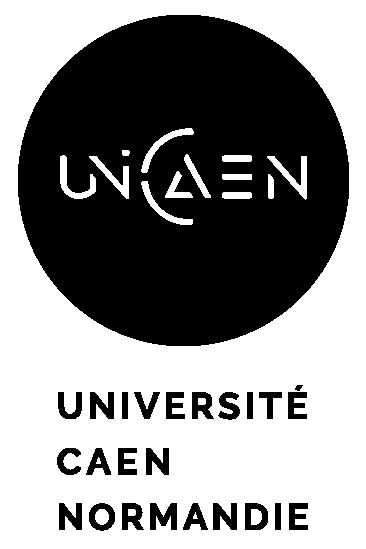
\includegraphics{images/logounicaen.png}\par\vspace{1cm}
    {\scshape\LARGE Rapport projet conception logicielle \par}
    \vspace{1cm}
    {\scshape\Large PyPuzzle\par}
    \vspace{1cm}
	{\Large Romuald GAFFE\par}
	{\Large Yanis COSNEFROY\par}
	{\Large Nguyen Phuong Vy VU\par}
	{\Large Alexandre BOURGOIN\par}
    \vspace{1cm}
	{\large \today \par}
\end{titlepage}

\tableofcontents
\part{Objectifs du projet}
\section{Présentation du concept}
Tout d'abord, nous avons choisi de créer un puzzle block puisque nous avions plus d'affinité et d'idées en rapport avec ce sujet. Nous voulions que ce jeu soit simple d'utilisation afin que tout le monde puisse y jouer. Le jeu que nous avons développé est composé de 4 modes de jeux, le premier étant le mode de jeu solo, il se présente sous forme d'une grille carré de 10 cases de côté. Le joueur obtient 3 pièces à placer sur la grille tirées aléatoirement parmi un total de 30 pièces(toutes orientations inclus). Les pièces qui apparaissent doivent toutes être placés dans la grille avant que les suivantes soit tirés. Si le tirage courant du joueur ne peut pas être placé alors un écran de fin de jeu s'affiche, montrant le score de la personne. Sur ce menu, le joueur aura la possibilité de retourner au menu principal ou de recommencer une partie. Ensuite le jeu se compose d'un mode multijoueur. Le premier étant contre une intelligence artificielle ayant le même mode de fonctionnement que le mode solo. Seul le score actuel de l'intelligence artificielle figure sur l'écran du joueur afin d'éviter d'en copier la stratégie. Le second mode multijoueur est, lui, un mode joueur contre joueur en local sur une même machine. Les grilles des joueurs s'affichent l'une après l'autre afin de limiter, de même, l'imitation de la stratégie adverse. Le dernier mode de jeu est un mode joueur contre joueur également mais en ligne où le but est de faire le plus de points.
\section{Cahier des charges}
Comme dit précédemment, nous voulions que le jeu soit simple d'utilisation afin qu'il puisse être accessible au plus grand nombre, nous voulions également que le jeu puisse être joué peu importe si on est seul ou à plusieurs, pour cela, nous avons décidé d'implémenter en accord avec le sujet du projet:
\begin{itemize}
	\item 4 modes de jeu: 
	\begin{itemize}
		\item Mode de jeu solo.
		\item Mode de jeu multijoueur joueur contre une intelligence artificielle.
		\item Mode de jeu multijoueur joueur contre joueur en local.
		\item Mode de jeu multijoueur joueur contre joueur en ligne.	
	\end{itemize}
	\item Un système de tirage pseudo-aléatoire des pièces.
	\item Une interface simple et ergonomique pour que l'utilisateur ne se perde pas.
	\item Un programme divisé en plusieurs modules.
\end{itemize}


\section{Exemples du jeux publiés}
Voici plusieurs block-puzzle provenant de jeux.fr, et des applications pour android: \\
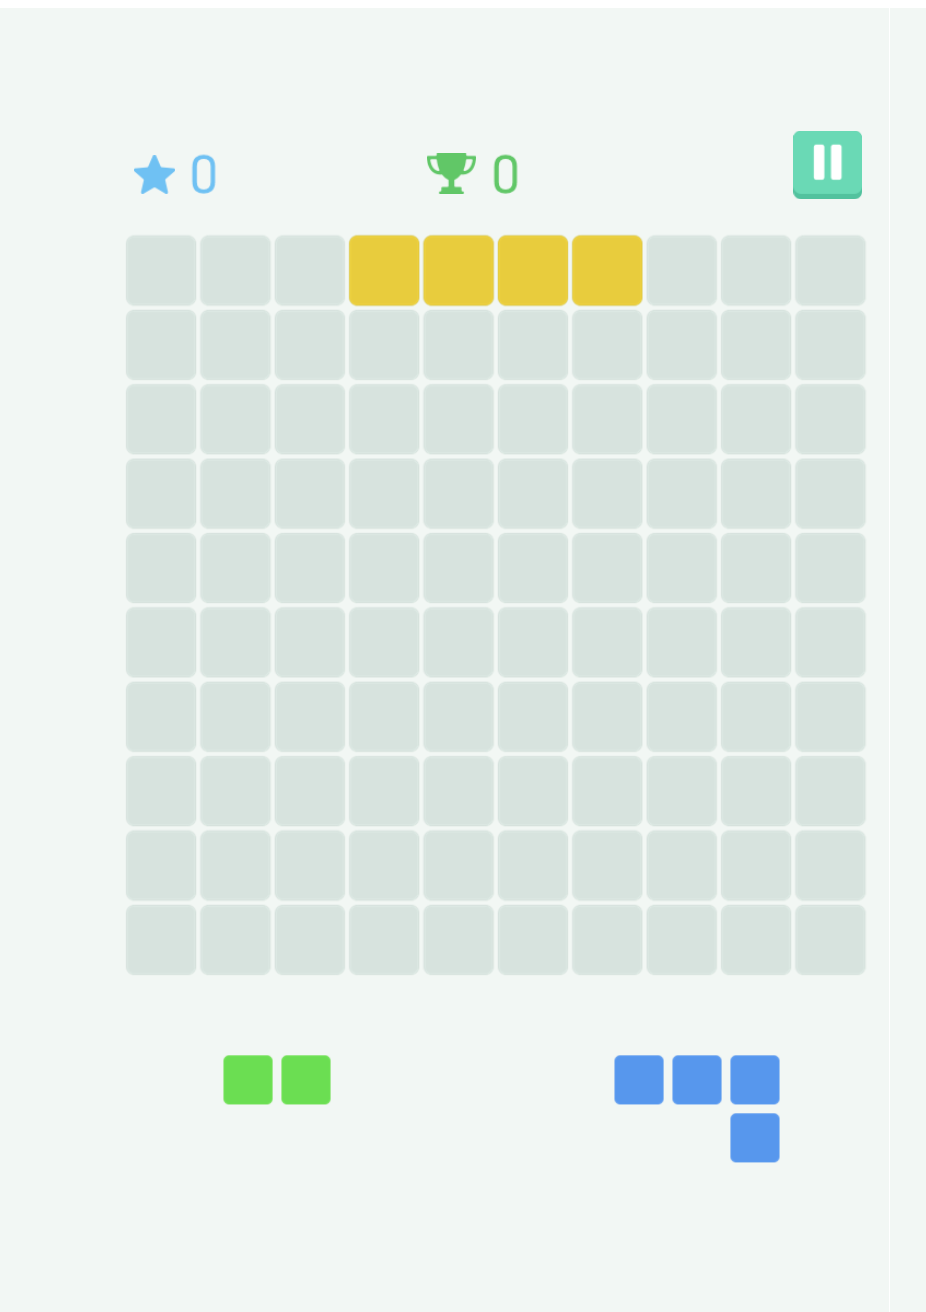
\includegraphics[height=180px]{images/jeuxPublie1.png}
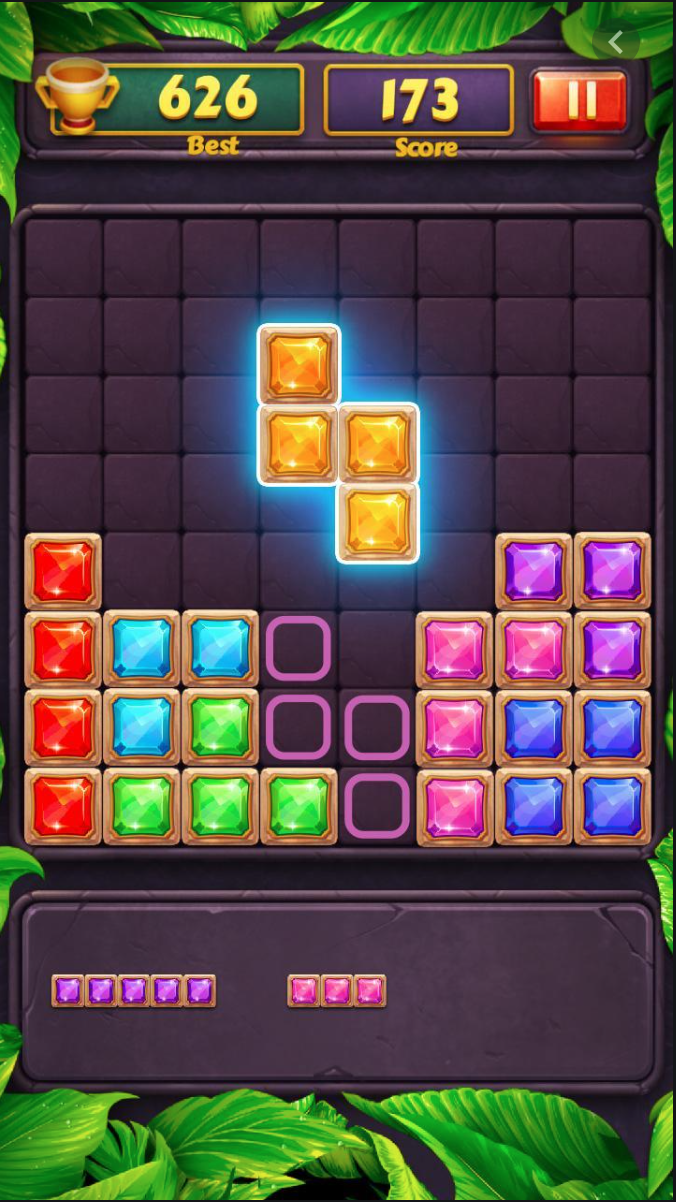
\includegraphics[height=180px]{images/jeuxPublie2.png}
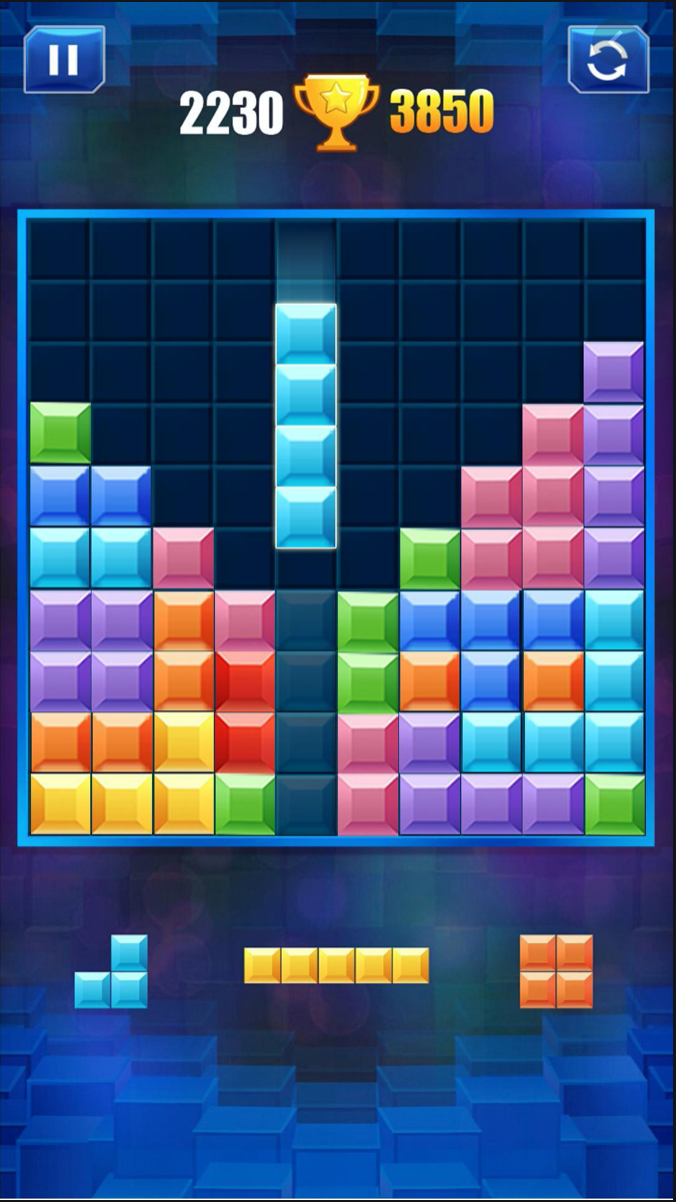
\includegraphics[height=180px]{images/jeuxPublie3.png}\\

On peut y retrouver les mêmes caractéristiques que notre projet. Notre projet a été conçu sur une base classique de block-puzzle qui réunit ces trois images montrées précédemment. Les différences entres ces block-puzzles et le nôtre sont l'aspect graphique ainsi que la sauvegarde du meilleur score établis sur le jeu par le joueur. On peut constater à l'essai de notre block-puzzle uniquement l'apparition des scores qui vont être actifs en fonction du jeu du joueur. Cependant nos règles sont un peu différentes par rapport au jeu déjà publié.
\part{Fonctionnalités implémentés}
\section{Mode solo}
\begin{wrapfigure}{R}{0.35\textwidth}
    \centering
    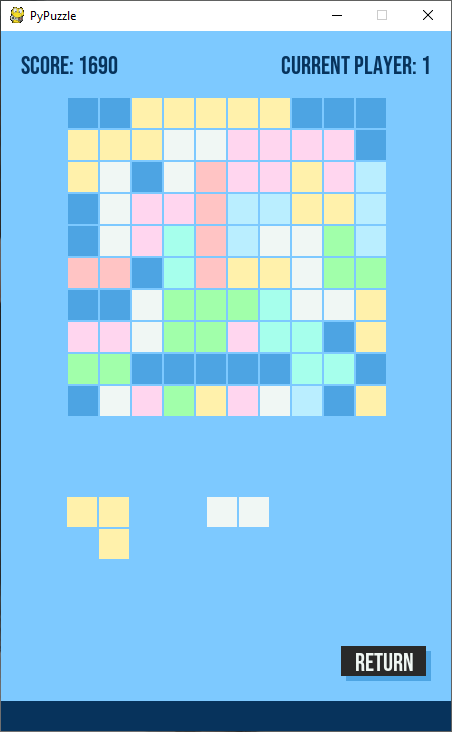
\includegraphics[width=0.3\textwidth, trim=0pt 0pt 0pt 30pt]{images/3-ingame.png}
    \caption{Gameplay solo}
\end{wrapfigure}
Tout d'abord la structure du jeu en mode solo est une structure de jeu plutôt classique comme on peut le voir dans l'image présente ci-dessous :\\

Comme on peut le constater à l'image du projet, il y a une grille placée au centre de la fenêtre qui possède une taille fixe. Autour de cette grille, va se trouver des informations essentielles pour le joueur comme son score actuel qui est placé en haut à gauche de la fenêtre. À droite, va se trouver le joueur qui joue. En dessous de la grille, on va retrouver les 3 pièces que le joueur devra placer sur la grille. Enfin, tout en bas à droite, il va y avoir un bouton pour permettre à l'utilisateur de retourner au menu du jeu. \\

Ensuite, les règles du jeu vont s'appliquer au fur et à mesure du jeu du joueur. Quand un block sera placé dans la grille, il va y avoir un ajout de 30 points à son score. Et dès qu'une ligne ou une colonne sera remplie, il va y avoir une disparition de la ligne ou de la colonne voir même les deux si les conditions sont réunies. Le bonus de point sera alors de 100 points lorsqu'une ligne ou une colonne est construite par l'utilisateur. Le joueur ne peut pas mettre sa partie en pause. Cependant, il n'y a pas de limite de temps. Dès que les trois blocs sont placés dans la grille, trois autres bloques vont réapparaître avec une probabilité de difficultés qui est calculée en fonction du score. \\

\begin{wrapfigure}{L}{0.35\textwidth}
    \centering
    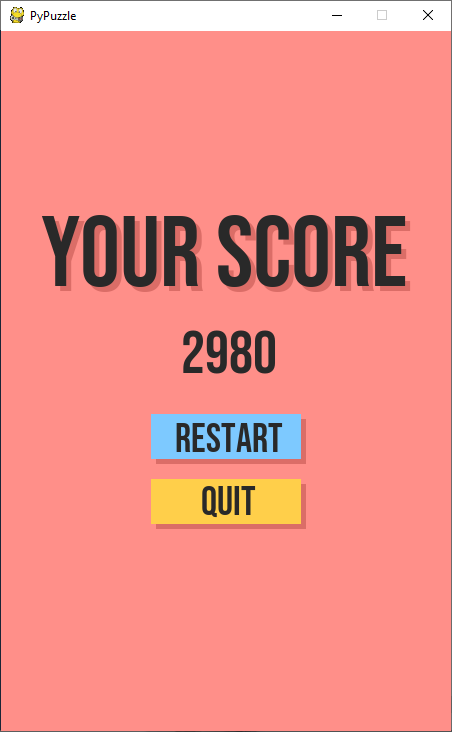
\includegraphics[width=0.3\textwidth, trim=0pt 0pt 0pt 50pt]{images/4-end.png}
    \caption{Gameplay solo}
    \vspace{-20pt}
\end{wrapfigure}

Enfin, si je le joueur perd en étant bloqué sur le placement impossible d'une pièce dans la grille, alors le jeu s'arrêtera et affichera un Game Over montré ci dessous avec les information de jeu du joueur : \\

Comme on peut le voir sur cette photo, le score du joueur est affiché. Afin d'éviter au joueur de repartir dans le menu pour relancer une partie, il a la possibilité de la relancer directement grâce au bouton "restart". Il a aussi la possibilité de quitter le jeu en cliquant sur le bouton "quit". Si le joueur veut retourner au menu, alors il devra d'abord recommencer une partie et cliquer sur le bouton "return" se trouvant en bas à droite de la fenêtre. 

\pagebreak

\section{Mode multijoueur}
\begin{wrapfigure}{R}{0.35\textwidth}
    \centering
    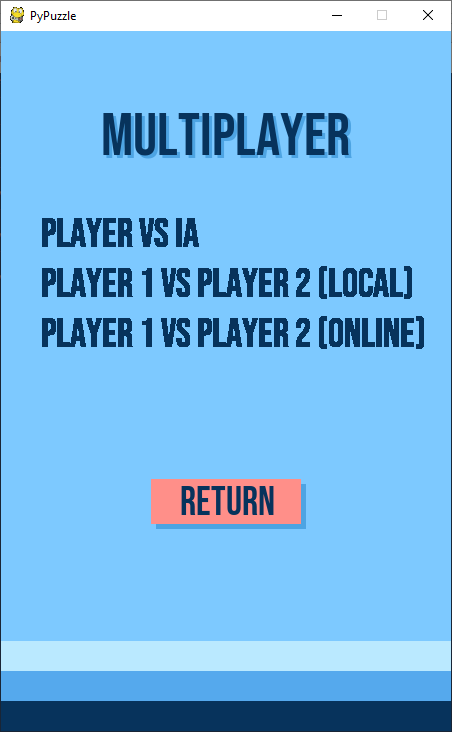
\includegraphics[width=0.3\textwidth, trim=0pt 0pt 0pt 150pt]{images/2-menumulti.png}
    \caption{Menu multijoueur}
    \vspace{-20pt}
\end{wrapfigure}
Différents modes de multijoueur sont présents dans ce projet. On peut y retrouver un multijoueur où un joueur réel va jouer contre une intelligence artificielle, un multijoueur où deux joueurs vont s'affronter. Et enfin un multijoueur en réseau où deux joueur vont pouvoir s'affronter sur deux écrans séparés. En dessous se trouve une image représentant le menu du multijoueur. On peut également y retrouver la possibilité d'un retour au menu principal dans le menu si le joueur veut jouer seul.\\


\subsection{Joueur vs Intelligence artificielle}
\begin{wrapfigure}{L}{0.35\textwidth}
    \centering
    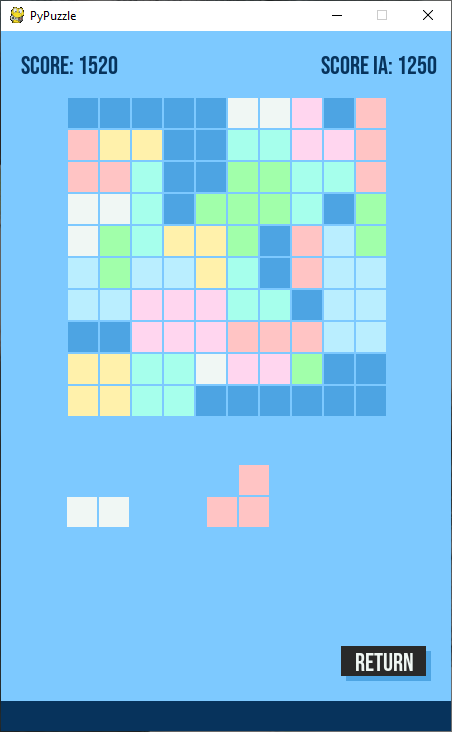
\includegraphics[width=0.3\textwidth, trim=0pt 0pt 0pt 30pt]{images/3-playwithai.png}
    \caption{Joueur vs IA}
    \vspace{-10pt}
\end{wrapfigure}
Tout d'abord, il faut savoir que le mode multijoueur avec le joueur contre l'intelligence artificielle se joue comme le mode solo. Le joueur va pouvoir jouer comme il voudra. Il n'aura pas accès à la grille de l'intelligence artificielle pour éviter la tricherie. L'utilisateur va avoir comme information sa grille, ses points, les points de son adversaire. Le joueur et l'intelligence artificielle vont tout les deux avoir les mêmes blocs pour que la difficulté soit la même de chaque côté. Le joueur va pouvoir retourner au menu si il le souhaite, toujours grâce au bouton se trouvant en bas à droite. Ci dessous, va se présenter une photo de la grille du jeu avec les différentes informations énoncées précédemment que le joueur va avoir.\\

\begin{wrapfigure}{R}{0.35\textwidth}
    \centering
    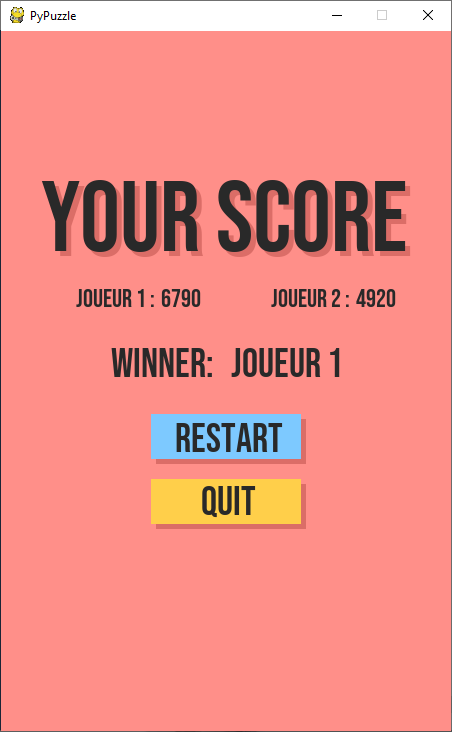
\includegraphics[width=0.3\textwidth, trim=0pt 0pt 0pt 30pt]{images/4-endmulti.png}
    \caption{Fin du jeu multi}
\end{wrapfigure}
Ensuite les règles du jeu sont les mêmes que pour le solo. Il n'y a pas de mise difficultés pour qui que ce soit car si l'un rempli une ligne ou une colonne, l'autre ne va pas recevoir de pièce qui peut le mettre en difficulté. Ici il y a juste une concurrence au niveau des points qui va justement permettre de départager la victoire entre le joueur et l'intelligence artificielle.\\

Enfin, si je le joueur perd en étant bloqué sur le placement impossible d'une pièce dans la grille, alors le jeu s'arrêtera et affichera un Game Over montré ci dessous avec les information de jeu du joueur. Si le jeu ne s'arrête pas c'est qu'il y a encore une possibilité de jouer.  \\

Comme on peut le voir sur cette photo, le score du joueur ainsi que celui de l'intelligence artificielle sont affiché. De plus on a décidé de rajouter une ligne pour faire ressortir le gagnant de la partie. Dans cette image, Player1 est le joueur se trouvant derrière l'écran et Player2 est l'intelligence artificielle. Afin d'éviter au joueur de repartir dans le menu pour relancer une partie, il a la possibilité de la relancer directement grâce au bouton "restart". Il a aussi la possibilité de quitter le jeu en cliquant sur le bouton "quit". Si le joueur veut retourner au menu, alors il devra d'abord recommencer une partie et cliquer sur le bouton "return" se trouvant en bas à droite de la fenêtre. 

\subsection{Joueur vs Joueur en local}
Le concept est le même que celui contre l'intelligence artificielle, mais cette fois-ci il se fera contre un autre joueur sur un même ordinateur, chaque joueur joue l'un après l'autre, le but étant de pouvoir placer les pièces tirées le plus longtemps possible, le premier à ne plus pouvoir placer son tirage se voit perdre. Le nombre de points n'est donc pas très important à prendre en compte dans ce mode de jeu. \\

Il y a toujours la possibilité de quitter la partie à tout moment avec le bouton "return" situé en bas à droite.
\subsection{Joueur vs Joueur en ligne}
Le mode de jeu en ligne se démarque un peu des autres modes de jeu multijoueur pour se rapprocher un peu plus du mode de jeu solo puisque le but ici est d'avoir le meilleur score, le tirage des deux joueurs est indépendant, ce qui ajoute une part de chance à la partie. Dans ce mode de jeu, si un joueur perds, l'autre joueur continue de jouer quand même, la partie n'est réellement fini que quand les deux joueurs ne peuvent plus jouer.


\part{Éléments techniques}

\section{Les pièces}
Les pièces sont représentés grâce à deux classes, il y a d'abord la classe \textbf{\textit{Pieces}} qui a comme propriété un tableau à deux dimensions, chaque lignes représentes une pièce différente et chaque colonne représente une "couche" de la pièce, comme toutes les pièces rentrent dans un carré de 5 par 5, il y a donc 5 couches. Une couche est une chaîne de caractère contenant des 0 et des 1. Chaque 1 représente une case constituant la pièce et les 0 représentent le vide. L'objet \textbf{\textit{Pieces}} est également chargé du tirage des pièces grâce aux propriétés \textbf{\textit{history}} où sont stocké les prochaines pièces tirées ainsi que la méthode \textbf{\textit{alea}} qui est la méthode de tirage pseudo-aléatoire. \\

La pièce en elle-même est représentée par la classe \textbf{\textit{Piece}} qui hérite de \textbf{\textit{Pieces}}, elle contient comme propriété sa couleur, un numéro correspondant à sa place dans le tableau \textbf{\textit{pieces}} contenant tous les pièces vu précédemment, sa position sur l'affichage quand elle est affichée dans le tirage ou déplacée par l'utilisateur, un booléen qui contient \textbf{\textit{True}} si la pièce est actuellement saisi par l'utilisateur et \textbf{\textit{False}} si elle ne l'est pas. La couleur des pièces dépend de la valeur de la chaîne de caractère de représentation de la pièce, par défaut nous avons vu que les couches de la pièces sont représentés par des 1 et des 0, la méthode \textbf{\textit{applyColor}} va changer chaque couche de la pièce en entier et la multiplier par la valeur correspondant à la couleur voulu. Cependant la passage de la chaîne de caractère à un entier va "dégrader" la pièce puisque tous les 0 situés avant les 1 dans la chaîne de caractère vont être supprimé, pour remédier à cela, il existe une autre méthode: \textbf{\textit{repair}} qui permet de rajouter à nouveau les 0 et donc "réparer" la pièce.

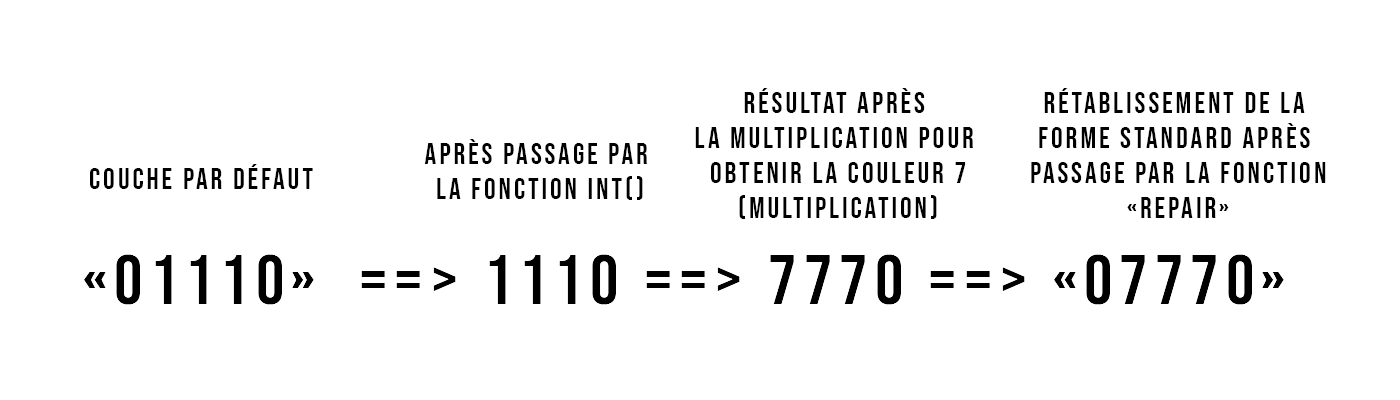
\includegraphics{images/schema_piece.png}

\section{La grille}
La grille est mise sous la forme d'un objet contenant comme propriétés sa taille, une grille où on placera les pièces, un objet \textbf{\textit{Pieces}} qu'on a décrit précédemment ainsi qu'un tableau où sont listés les lignes et colonnes complétées dans la grille.

L'objet \textbf{\textit{Grid}} contient également des méthodes permettant de la modifier ou de voir son état:
\begin{itemize}
	\item \textbf{\textit{init}} : Cette méthode permet d'initialiser la grille c'est à dire ajouter les listes correspondant aux colonnes avec la taille spécifiée.
	\item \textbf{\textit{print}} : Permet d'avoir l'état de la grille affichée dans la console.
	\item \textbf{\textit{definePhysicalLimits}} : Permet d'ajouter tout autour de la grille des 1 afin d'empêcher le joueur de placer des pièces en dehors de la grille.
	\item \textbf{\textit{isPiecePlaceable}} : Permet de voir si une pièce peut être placée à des coordonnées données.
	\item \textbf{\textit{putPiece}} : Permet de placer une pièce dans la grille.
	\item \textbf{\textit{isThereAlignment}} : Permet d'ajouter à la propriété \textbf{\textit{linesCompleted}} les lignes et colonnes complétés.
	\item \textbf{\textit{eraseAlignment}} : Supprime les alignements dans la grille.
	\item \textbf{\textit{isDrawPlaceable}} : Vérifie si le tirage d'un joueur donné peut être placé dans la grille.
\end{itemize}

\section{L'aléatoire}


\section{L'intelligence artificielle}
L'intelligence artificielle se présente comme une dérivée de la classe \textbf{\textit{Player}} car elle a les mêmes priorités qu'un joueur comme ses points ou un tirage, le changement se fait avec la méthode \textbf{\textit{determineWhatToPlay}} qui retourne le placement le plus judicieux à effectuer sous la forme d'un tableau contenant le poids attribué au mouvement, les coordonnées ou il doit se faire et la pièce à jouer. \\

La méthode va tester pour chaque case de la grille si chaque pièce peut être placée, dans ce cas le poid du mouvement sera incrémenté de 1, ensuite si le mouvement créer une ou plusieurs lignes, il rajoutera au poids le nombre de lignes remplies. Pour deux poids égaux, ce sera la mouvement le plus en bas à droite de la grille qui sera compté. \\

Sur 100 parties solo jouées par l'intelligence, voici les statistiques que nous avons pu récolter(via le programme "IAStats.py" situé à la racine du répertoire git): \\

Nombre de rounds:\\
Moyenne: 51.08\\
Maximum: 86\\
Minimum: 26\\

Nombre de points:\\
Moyenne: 2317.4\\
Maximum: 4400\\
Minimum: 780\\


\section{Le réseau}
Le jeu PyPuzzle possédé par le joueur ne fait office que de client pour le jeu en réseau donc les personnes possédant le jeu n'auront pas la possibilité d'héberger leur propre partie à partir de leur client mais devront rejoindre un serveur. \\

La partie client est un jeu solo classique comme décrit précédemment, le client va recevoir à chaque tour de boucle l'état de la partie qui peut être soit:
\begin{itemize}
	\item "wait" : En attente d'un second joueur.
	\item "running" : La partie est en cours.
	\item "quit" : Un des client a quitté la partie, l'autre client retourne au menu principal.
	\item "gameover" : Un des deux joueurs a fini de jouer.
\end{itemize}
Il va également demander l'état des points des deux joueurs afin de les afficher. Tout se fait grâce à l'objet \textbf{\textit{Network}} permettant de simplifier la connexion et l'envoi de donnée au serveur.\\

Côté serveur, chaque connexion client incrémente une variable \textbf{\textit{idCount}} qui va permettre d'attribuer un joueur se connectant à une partie. Chaque partie dispose d'un \textbf{\textit{gameID}} qui permet de l'identifier dans un dictionnaire: \textbf{\textit{games}}. Chaque partie de jeu dans le dictionnaire contient le nombre de points des deux joueurs ainsi que l'état dans lequel est la partie. Lorsque qu'une partie se termine, les joueurs se déconnectent, \textbf{\textit{idCount}} est décrémenté et les données de la partie dans le dictionnaire sont supprimés afin de libérer de la mémoire.


\section{L'interface graphique}
Pour l'interface du jeu, on utilise \textbf{\textit{Pygame}}, une bibliothèque graphique dédiée aux jeux vidéos. 
Pygame n'est pas fourni avec Python. Donc, pour jouer, vous devrez télécharger et installer Pygame à la place. Pour appliquer Pygame:
\begin{lstlisting}
    import pygame @\color{blue}as@ pg
\end{lstlisting}

On va utiliser pygame pour faire et design l'interface du jeu, pas utiliser les images déjà faits et les mettre dans le jeu.
Et on va appliquer en même méthode pour faire le menu démarrer, le menu multijoueur et le menu de la fin du jeu.

\subsection{Le menu}
D'abord, il faut faire un réglage des tailles des positions. \textbf{\textit{pygame.Rect()}} n'est pas dessiner un rectangle, juste déterminé les tailles et les positions d'un rectangle.
\begin{lstlisting}
    #tailles de fenetre
    SCREENHEIGHT = 700
    SCREENWIDTH = 450
    screensize = (SCREENWIDTH, SCREENHEIGHT)
    #positions de la grille
    boardX = 65
    boardY = 65
    #tailles et positions des boutons
    soloButtonRect = pg.@\color{blue}Rect@(150, 318, 150, 50)
    multiButtonRect = pg.@\color{blue}Rect@(150, 383, 150, 50)
    quitButtonRect = pg.@\color{blue}Rect@(150, 448, 150, 45)
\end{lstlisting}

Pour commencer le jeu, on doit appeler la fonction \textbf{\textit{pygame.init()}}, elle doit être appelée en premier pour que de nombreuses fonctions Pygame fonctionnent
\begin{lstlisting}
    pg.@\color{blue}init()@
\end{lstlisting}

Ensuite, on doit construit un boucle pour tout le menu. Si une boucle est toujours vrai, alors elle fonctionne pour toujours.
\begin{lstlisting}
    def menu():
    doContinue = True
    while doContinue:
        for event in pg.event.get():
            if event.@type@ == pg.QUIT:
                fnc.quitGame() #dans function.py pour quitter
\end{lstlisting}

Puis, on ajoute des boutons, on utilise \textbf{\textit{.collidepoint()}} pour déterminer les positions des boutons.
\begin{lstlisting}
                elif event.@type@ == pg.MOUSEBUTTONDOWN:
                if soloButtonRect.@\color{blue}collidepoint@(@\color{blue}event.pos@):
                    solo() #autre menu pour basculer entre eux
                if multiButtonRect.@\color{blue}collidepoint@(@\color{blue}event.pos@):
                    multiMenu() #autre menu pour basculer entre eux
                if quitButtonRect.@\color{blue}collidepoint@(@\color{blue}event.pos@):
                    fnc.quitGame() #dans function.py pour quitter
        pg.display..@\color{blue}flip@() #pour mise a jour
\end{lstlisting}

Ensuite, on construit une interface d'affichage dans une autre fichier appelée \textbf{display.py}. 
Pour les textes, on utilise \textbf{\textit{pygame.font}} avec les sous-éléments \textbf{\textit{pygame.font.Font()}}, \textbf{\textit{"nom".render()}} et l'élement \textbf{\textit{"screen".blit()}}. 
Pour les rectangles (boutons), on utilise \textbf{\textit{pygame.draw.rect()}}.
Et pour colorer le fond, on utilise \textbf{\textit{"screen".fill()}}.

\begin{lstlisting}
    NAVY = (7, 51, 92)
    pg.font.@\color{blue}init()@
    bigFont = pg.font.@\color{blue}Font@('assets/BebasNeue-Regular.ttf', 100)
    pypuzzle = bigFont.@\color{blue}render@("PyPuzzle", True, NAVY)

    def displayMenu(win):
    win.@\color{blue}fill@(BACKGROUNDCOLOR)
    pg.draw.@\color{blue}rect@(win, BOARDCOLOR, (155, 323, 150, 45))
    pg.draw.@\color{blue}rect@(win, BOARDCOLOR, (155, 388, 150, 45))
    pg.draw.@\color{blue}rect@(win, BOARDCOLOR, (155, 453, 150, 45))
    #titre
    win.@\color{blue}blit@(pypuzzleShadow, (82, 170))
    win.@\color{blue}blit@(pypuzzle, (78, 165))
    #decoration
    pg.draw.@\color{blue}rect@(win, LIGHTBLUE, (0, 610, 450, 30))
    pg.draw.@\color{blue}rect@(win, BLUE, (0, 640, 450, 30))
    pg.draw.@\color{blue}rec@t(win, NAVY, (0, 670, 450, 30))
\end{lstlisting}

Pour les son, on utilise \textbf{\textit{pygame.mixer}} avec les sous-éléments \textbf{\textit{pygame.mixer.Sound()}}, \textbf{\textit{"nom".play()}} et \textbf{\textit{"nom".stop()}}.
Type de fichier est .wav (Les formats de fichiers audio pris en charge par Pygame sont MID, WAV et MP3.)
\begin{lstlisting}
    pg.mixer.@\color{blue}init@() #pour fonctioner
    soundMenu = pg.mixer.@\color{blue}Sound@("assets/menu.wav")
    soundMenu.@\color{blue}play@(-1, 0, 0)
\end{lstlisting}

On juste utilise une animation, c'est le survol quand on entre les boutons.
Ici, on utilise \textbf{\textit{pygame.mouse}} avec le sous-élement \textbf{\textit{pygame.mouse.get\_pos()}}.
pour déterminer les positions de la souris.
\begin{lstlisting}
    # HOVER
    pos = pg.mouse.@\color{blue}get\_pos()@
    if 340 + 85 > pos[0] > 340 and 615 + 30 > pos[1] > 615:
        pg.draw.@\color{blue}rect@(screen, dsp.YELLOW, (340, 615, 85, 30))
        screen.@\color{blue}blit@(dsp.returnMenuText, (354, 617))
    else:
        pg.draw.@\color{blue}rect@(screen, dsp.GRAY, (340, 615, 85, 30))
        screen.@\color{blue}blit@(dsp.returnMenuText1, (354, 617))
\end{lstlisting}

\subsection{Gameplay}


\part{Expérimentations et usages}
\section{Capture écrans}
Les captures ci-dessous rendront le joueur passionné de jouer au jeu.
\begin{enumerate}
    \item Menu démarrer avec animation de survol.\\
        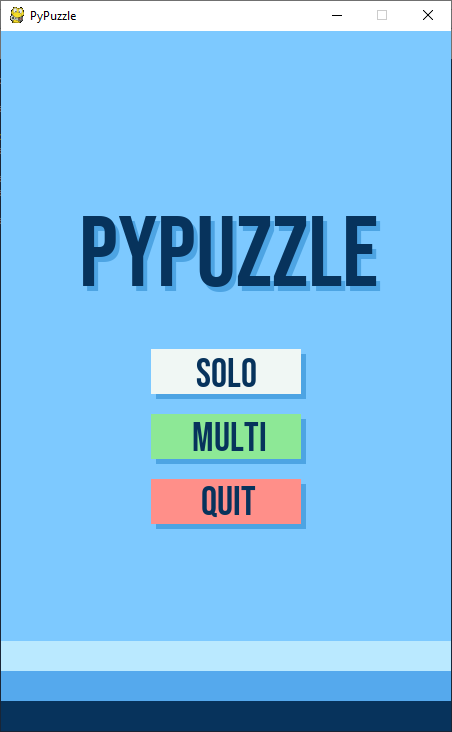
\includegraphics[scale=0.3]{images/1-menu.png}
        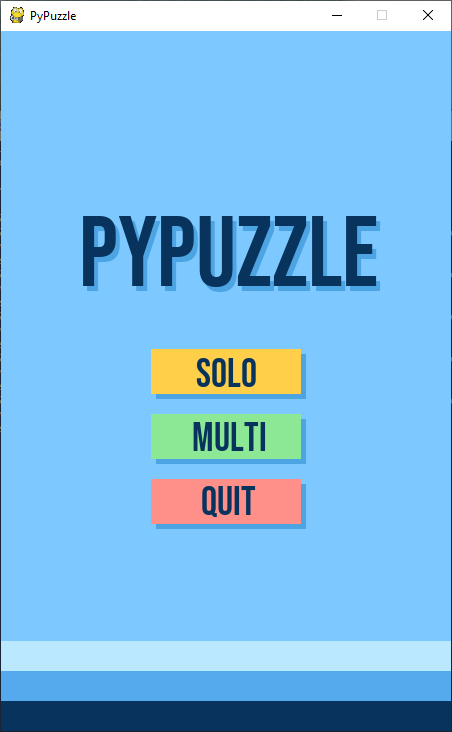
\includegraphics[scale=0.3]{images/1-ani.png}
    \item Menu multijoueur avec animation de survol.\\
        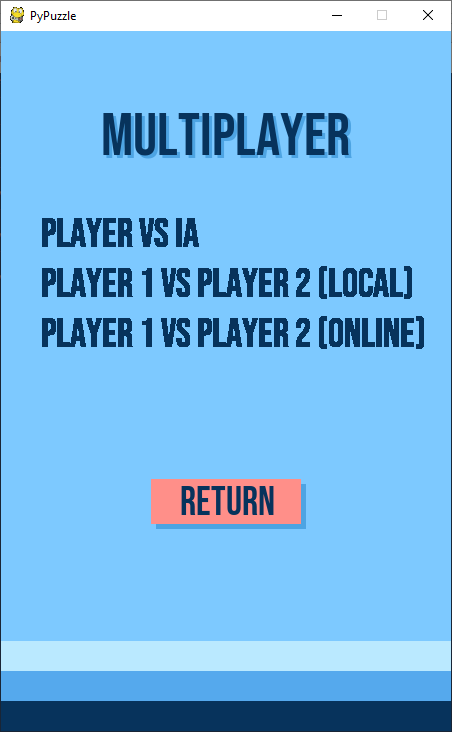
\includegraphics[scale=0.3]{images/2-menumulti.png}
        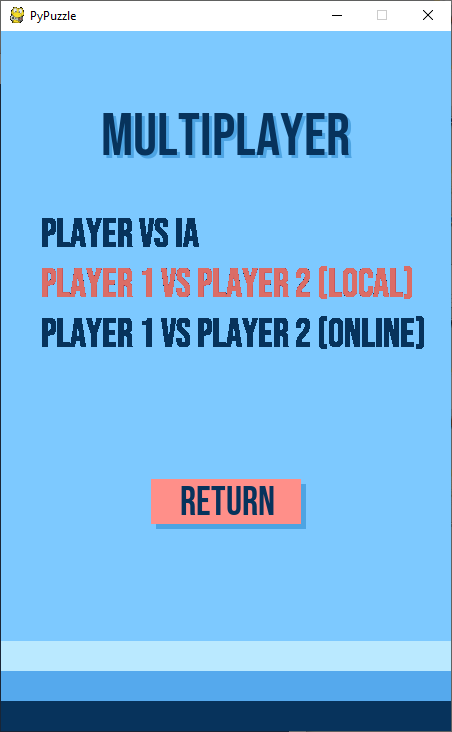
\includegraphics[scale=0.3]{images/2-ani.png}
    \item Gameplay (solo et multi). De nombreuses couleurs permettent au joueur de continuer et de ne pas s'ennuyer quand on joue.\\
        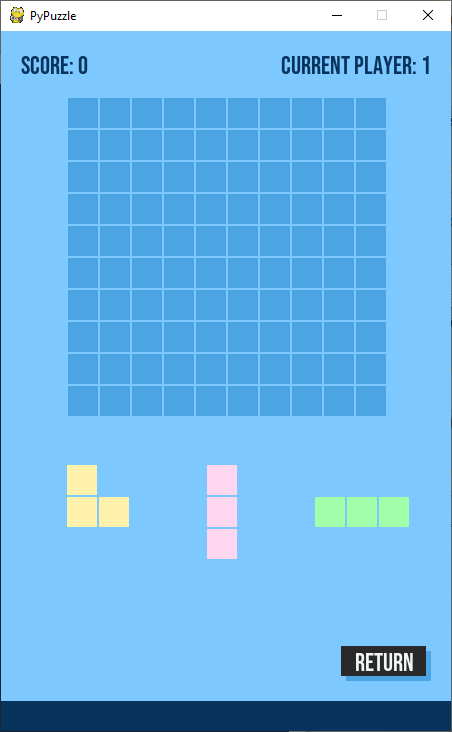
\includegraphics[scale=0.3]{images/3-ingamestart.png}
        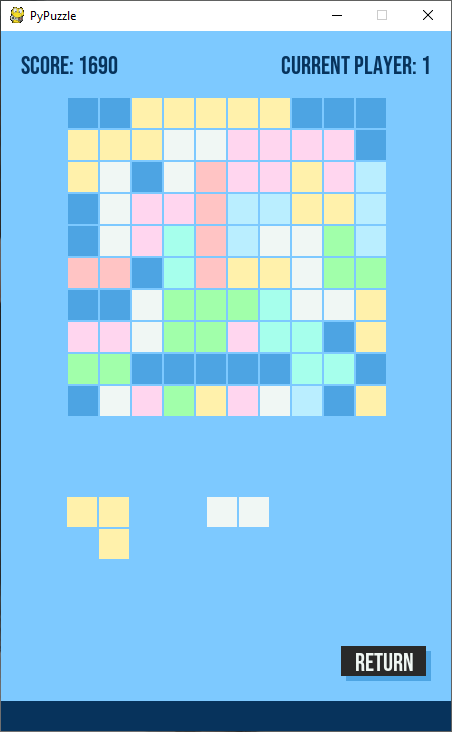
\includegraphics[scale=0.3]{images/3-ingame.png}
        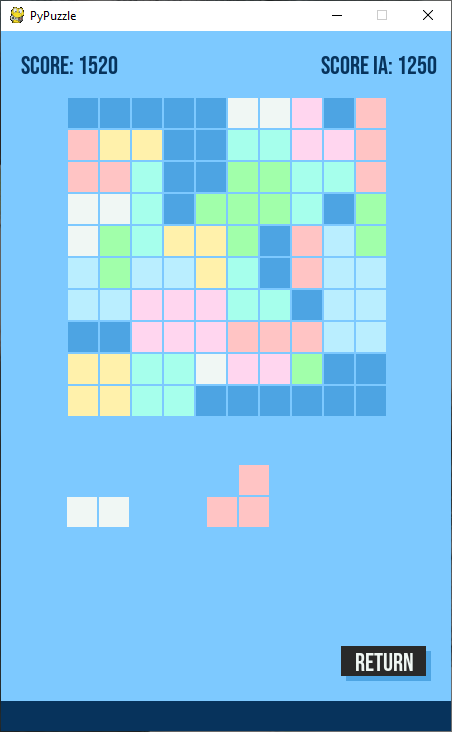
\includegraphics[scale=0.3]{images/3-playwithai.png}
    \item Fin du jeu avec animation de survol.\\
        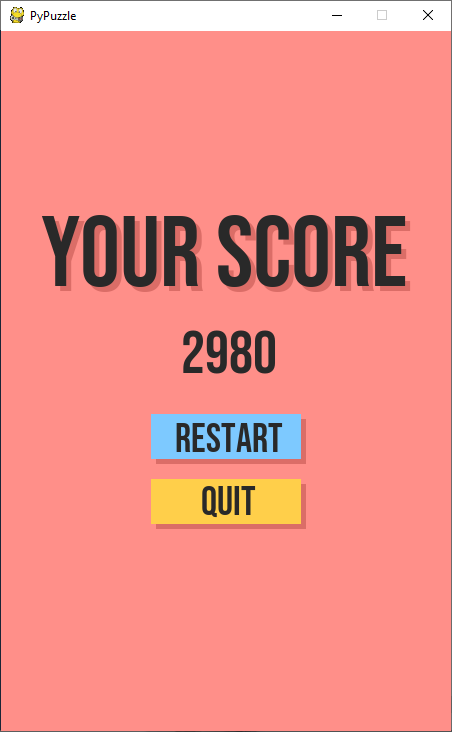
\includegraphics[scale=0.3]{images/4-end.png}
        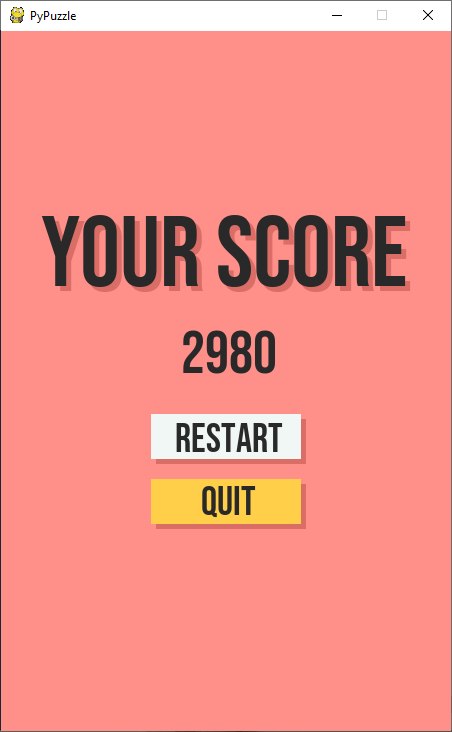
\includegraphics[scale=0.3]{images/4-endani.png}
        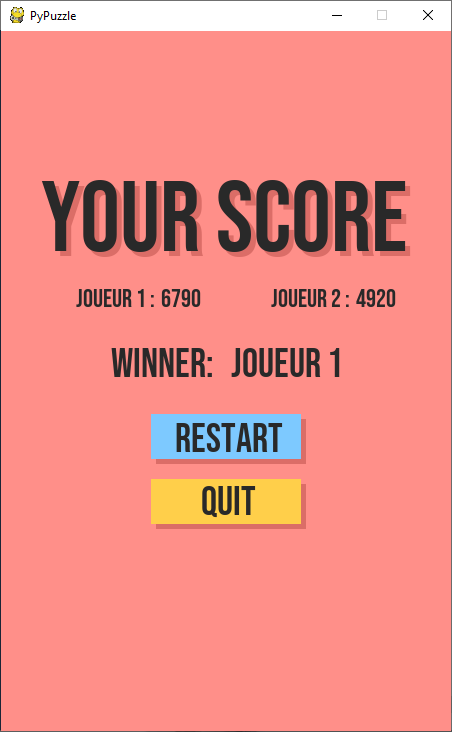
\includegraphics[scale=0.3]{images/4-endmulti.png}
\end{enumerate}


\section{Mesures de performance}

\subsection{Interfaces graphiques} 
Quelle est l'interface du jeu pour vous? Selon nous, après le contenu du jeu, l'interface du jeu est la plus importante pour attirer les joueurs.
C'est un jeu pour tout le monde, on choisit le minimalisme avec
une palette des couleurs pastels car ce sont des couleurs douces et pas sombres. 
Elle fait une atmosphère relaxée quand on joue. On échoue, mais sans s'énerver.\\

\begin{itemize} 
    \item Font: Bebas Neue Regular (Free Copyright)
    \item Couleur principale: \textbf{bleu(125, 201, 255)}
    \item Couleurs des pièces: les couleurs pastels\\
        
\includegraphics[scale=0.3]{images/palette1.png}
    \item Couleurs de menu\\
        
\includegraphics[scale=0.3]{images/palette2.png}
\end{itemize}

\subsection{Effet sonore}
On voulait ajouter de la musique à notre jeu, car on pensait que cela attirerait les joueurs. 
Comme la musique est quelque chose de très populaire à partir de maintenant, on pensait que les 
joueurs aimeraient qu'on ajoute de la musique au jeu que nous avons créé.\\

Au début du jeu, pas de bruit tonitruant, pas de son nerveux, on souhaite mettre le confort et la joie en premier en jouant. C'est pourquoi on choisit l'accord de base au piano C(Do) majeur.
Ensuite, le son des boutons est la note F(Fa) correspond à la première note de son du menu.
Puis, quand on joue, il n'y a pas de son de fond, il existe que le son des pièces pour que l'on se sente concentré. Il faut savoir que l'on n'oublie pas être en train de jouer au jeu donc le son du bongo apparait quand on drag and drop les pièces.
Enfin, on choisit l'accord guitare C(Do) mineur et on pense à créer une synchronisation de la musique.

\part{Organisation}

\begin{center}
\begin{tabular}{|c|c|c|}\hline   
Fonction/classe				&Fichier		  			&Personnes \\ \hline\hline
updates&      				pypuzzle.py&      			Alexandre\\\hline
updatesMultiLocal&     		pypuzzle.py&      			Alexandre\\\hline
menu&      					pypuzzle.py&      			Romuald, Vy, Yanis\\\hline
multiMenu&      			pypuzzle.py&      			Alexandre\\\hline
gameOverSolo&      			pypuzzle.py&      			Alexandre\\\hline
gameOverMulti&      		pypuzzle.py&      			Vy, Yanis\\\hline
solo&      					pypuzzle.py&      			Alexandre, Romuald, Yanis, Vy\\\hline
multiLocal&      			pypuzzle.py&      			Alexandre, Vy\\\hline
multiIA&      				pypuzzle.py&      			Alexandre, Vy, Romuald\\\hline
multiOnlineClient&      	pypuzzle.py&				Alexandre, Vy\\\hline
&      						server.py&     				Alexandre\\\hline
&							IAStats.py&					Alexandre \\\hline
displayMenu&      			modules/display.py&      	Vy\\\hline
displayMulti&      			modules/display.py&      	Vy\\\hline
displayBoard&      			modules/display.py&      	Alexandre, Vy\\\hline
displayDrawPieces&      	modules/display.py&      	Alexandre\\\hline
displayTexts&      			modules/display.py&      	Alexandre\\\hline
displayTextsIA&      		modules/display.py&      	Alexandre\\\hline
displayTextsOnline&      	modules/display.py&      	Alexandre\\\hline
displayGameOverSolo&      	modules/display.py&      	Alexandre, Yanis, Vy\\\hline
displayGameOverMulti&      	modules/display.py&      	Yanis, Vy\\\hline
displaygameOverMultiOnline& modules/display.py&      	Alexandre, Yanis, Vy\\\hline
displayWaitPlayers&      	modules/display.py&      	Alexandre\\\hline
&	      					modules/functions.py&      	Alexandre\\\hline
&      						modules/logicalgate.py&     Alexandre\\\hline
Grid&      					modules/grid.py&      		Alexandre, Yanis\\\hline
Network&      				modules/network.py&      	Alexandre\\\hline
Pieces&      				modules/pieces.py&      	Alexandre, Romuald\\\hline
Piece&      				modules/pieces.py&      	Alexandre\\\hline
Player&      				modules/player.py&      	Alexandre\\\hline
IA&      					modules/player.py&      	Alexandre\\\hline
\end{tabular}\end{center}

Numéros de téléphone: \\
Romuald GAFFE: \\
Yanis COSNEFROY:\\
Nguyen Phuong Vy VU:\\
Alexandre BOURGOIN: \


\part{Conclusion}
Pour conclure, nous voulons remercier Mme.LAMBERT de nous avoir encadré pendant les cours de travaux pratiques ainsi que M.BONNET pour ses cours. Merci d'avoir pris le temps de lire ce rapport. \\

\end{document}
